\section{Appendix: Composite Finite Element Analysis}

\subsection{Physics Models}

\begin{figure}[htp]
\centering
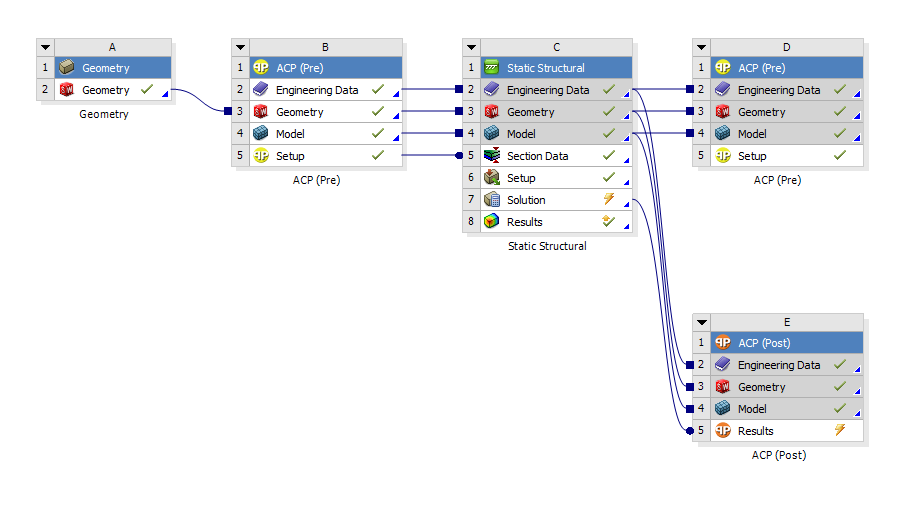
\includegraphics[width=1\textwidth]{./figures/fea/fea-project-schematic}
\caption{A schematic of the physics models used in this FEA.}
\label{fig:fea-project-schematic}
\end{figure}

\clearpage

\subsection{Material Data}

\begin{table}[htp]
    \centering
    \begin{tabular}{lcc}
        Property & Value & Unit \\ \hline
        
        Density & 800 & kg m$^{-3}$\\ 
        
        Young's Modulus X Direction & 2.31E+11 & Pa\\
        Young's Modulus Y Direction & 1.72E+09 & Pa\\
        Young's Modulus Z Direction & 1.72E+09 & Pa\\
        Poisson's Ratio XY & 0.35 &\\
        Poisson's Ratio YZ & 0.35 &\\
        Poisson's Ratio XZ & 0.35 &\\
        Shear Modulus XY & 7E+08 & Pa\\
        Shear Modulus YZ & 7E+08 & Pa\\
        Shear Modulus XZ & 7E+08 & Pa\\
        
        Tensile X Direction Stress Limit & 3.13E+08 & Pa\\
        Tensile Y Direction Stress Limit & 3.45E+07 & Pa\\
        Tensile Z Direction Stress Limit & 3.45E+07 & Pa\\
        Compressive X Direction Stress Limit & -1.57E+08 & Pa\\
        Compressive Y Direction Stress Limit & -1.73E+07 & Pa\\
        Compressive Z Direction Stress Limit & -1.73E+07 & Pa\\
        Shear XY Stress Limit & 6E+07 & Pa\\
        Shear YZ Stress Limit & 3.2E+07 & Pa\\
        Shear XZ Stress Limit & 6E+07 & Pa\\
        
        Tensile X Direction Strain Limit & 0.03 &\\
        Tensile Y Direction Strain Limit & 0.25 &\\
        Tensile Z Direction Strain Limit & 0.25 &\\
        Compressive X Direction Strain Limit & -0.015&\\
        Compressive Y Direction Strain Limit & -0.125 &\\
        Compressive Z Direction Strain Limit & -0.125 &\\
        Shear XY Strain Limit & 0.012 &\\
        Shear YZ Strain Limit & 0.011 &\\
        Shear XZ Strain  Limit & 0.012 &\\  
        
        Puck Material Classification & Carbon &\\
        Puck Compressive Inclination XZ & 0.3 &\\
        Puck Compressive Inclination YZ & 0.25 &\\
        Puck Tensile Inclination XZ & 0.35 &\\
        Puck Tensile Inclination YZ & 0.25 &\\
        
        Puck Interface Weakening Factor & 0.8 &\\
        Puck Degradation Parameter s & 0.5 &\\
        Puck Degredation Parameter M & 0.5 &\\
              
        
    \end{tabular}
    \caption{CFRP material properties used in \textit{ANSYS}.}
    \label{tab:ansys-material-properties}
\end{table}

\clearpage

\subsection{Geometry}

\begin{figure}[htp]
\centering
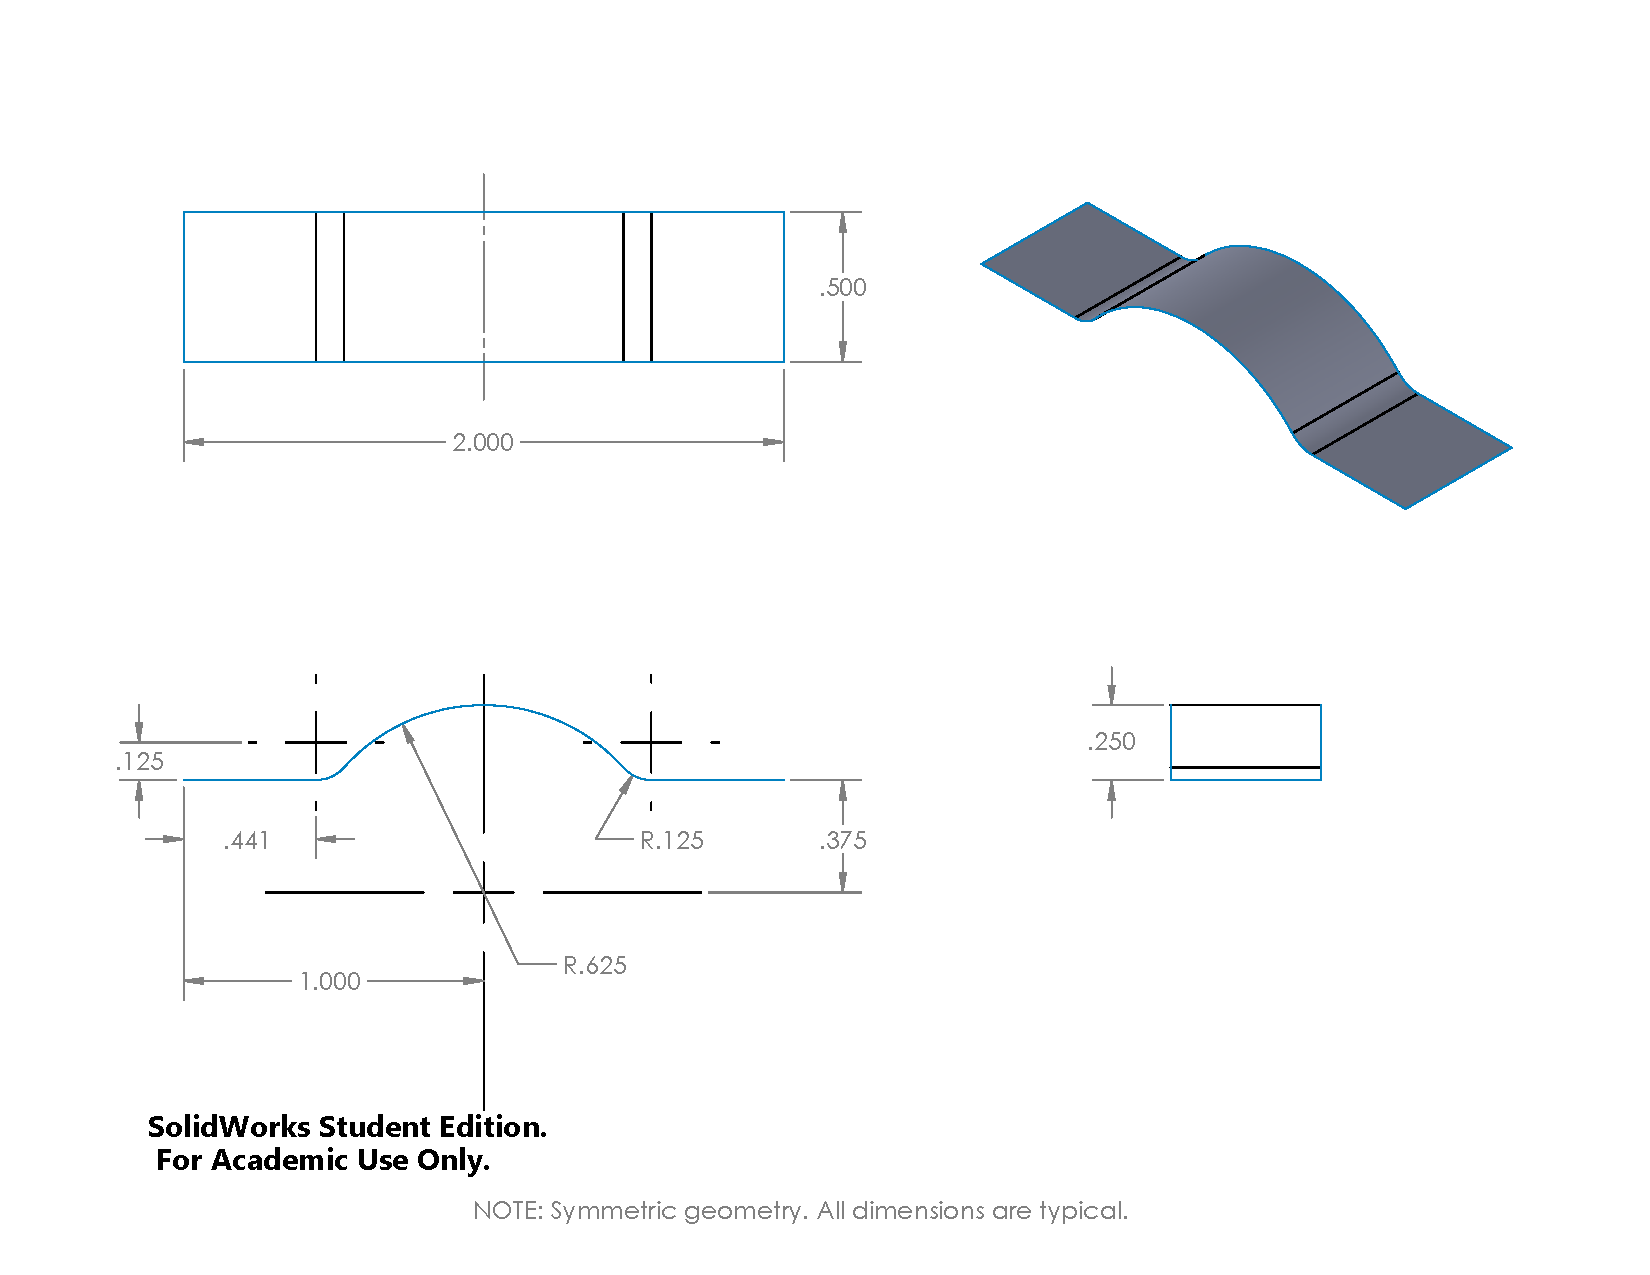
\includegraphics[width=1\textwidth]{./figures/fea/fea-surface-geometry}
\caption{A \emph{SolidWorks} drawing of the surface used for composite FEA.}
\label{fig:fea-surface-geometry}
\end{figure}

\subsection{Loads and Boundary Conditions}

\begin{figure}[htp]
\centering
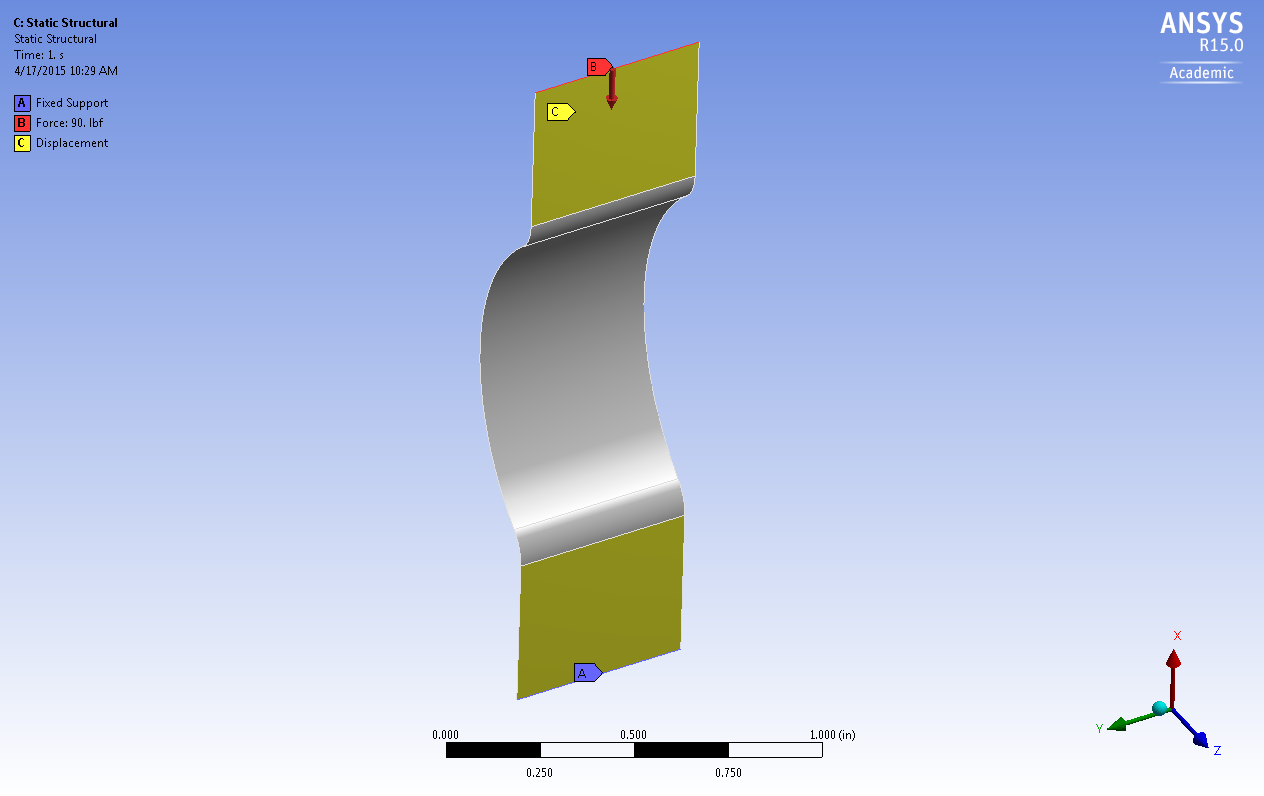
\includegraphics[width=1\textwidth]{./figures/fea/fea-mechanical-loads-bc}
\caption{The loads and boundary conditions applied to the surface geometry.}
\label{fig:fea-loads-bcs}
\end{figure}

\clearpage

\subsection{Meshing}

\begin{figure}[htp]
\centering
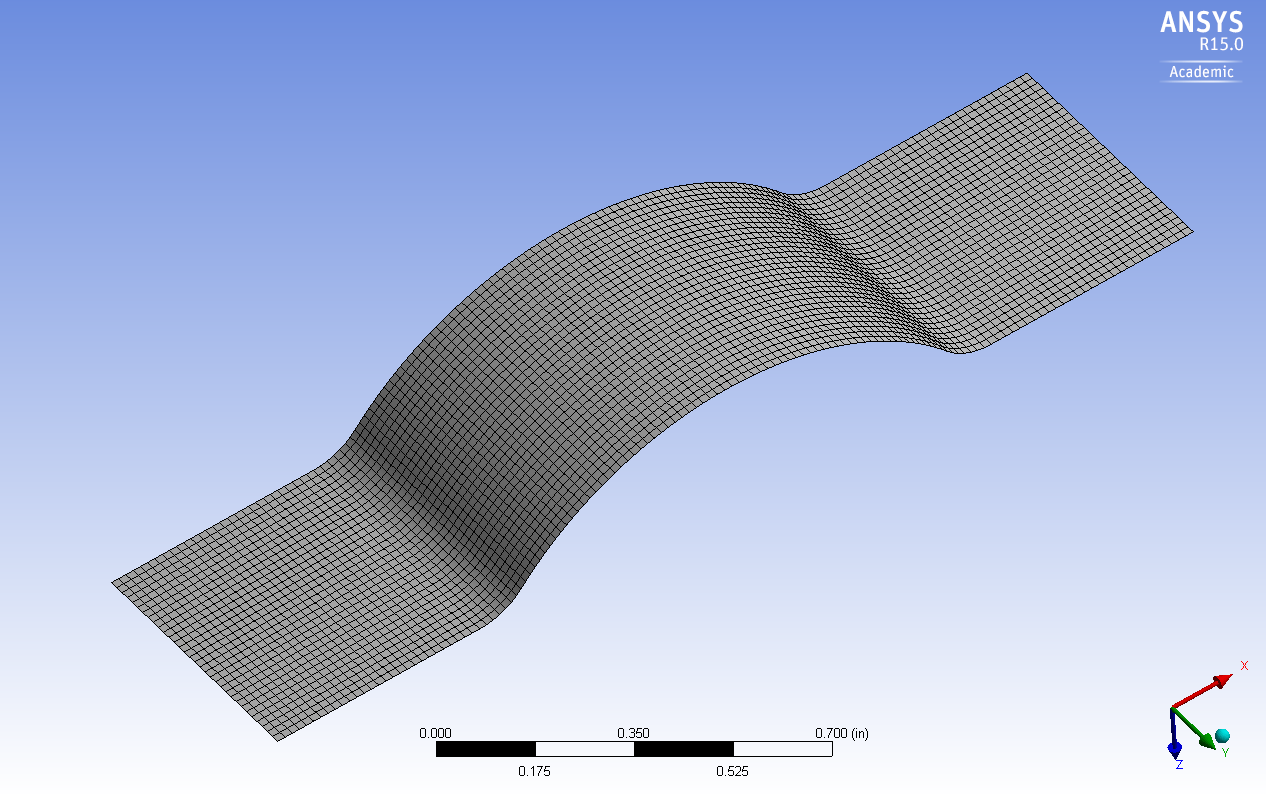
\includegraphics[width=1\textwidth]{./figures/fea/fea-mechanical-mesh-surface}
\caption{An overview of the mesh applied in \textit{ANSYS Mechanical}.}
\label{fig:fea-mechanical-mesh-surface}
\end{figure}

\begin{figure}[htp]
\centering
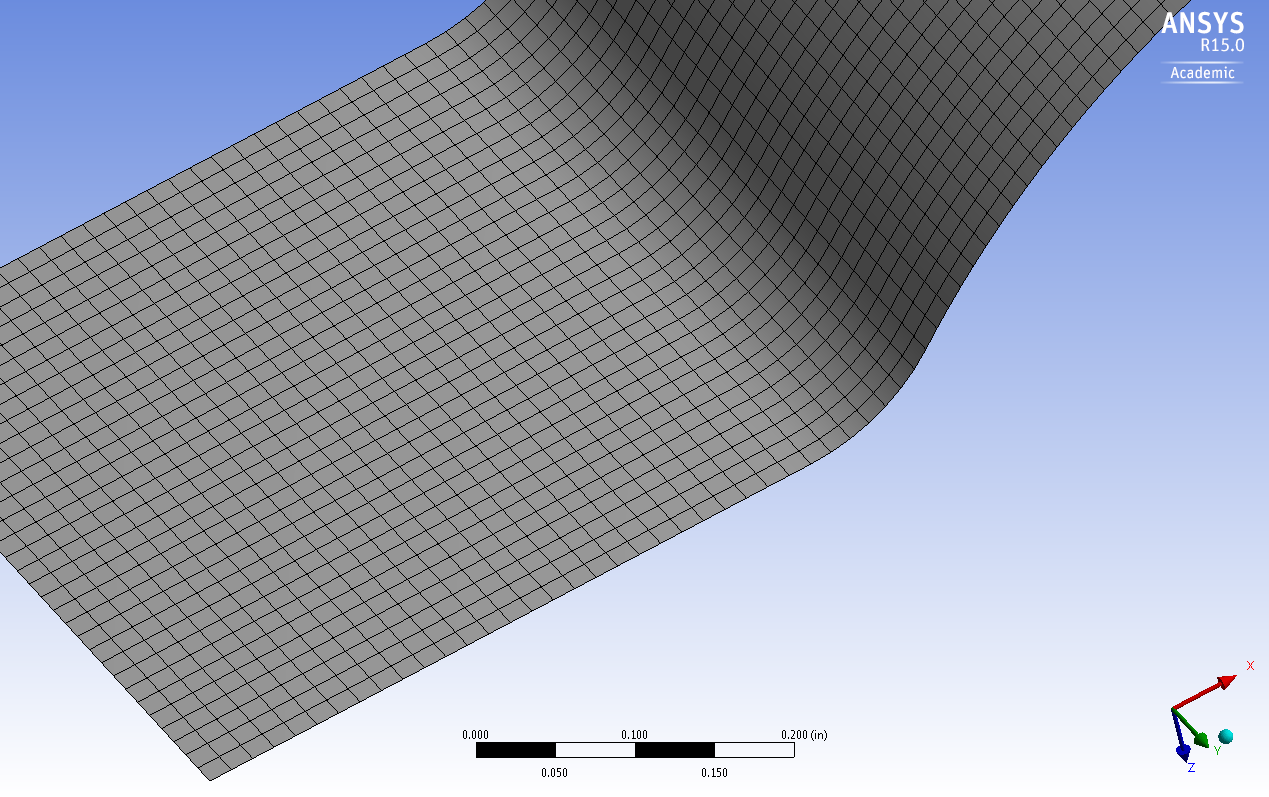
\includegraphics[width=1\textwidth]{./figures/fea/fea-mechanical-mesh-closeup}
\caption{A close-up of the mesh showing its size dependency based on feature geometry.}
\label{fig:fea-mechanical-mesh-closeup}
\end{figure}

\begin{figure}[htp]
\centering
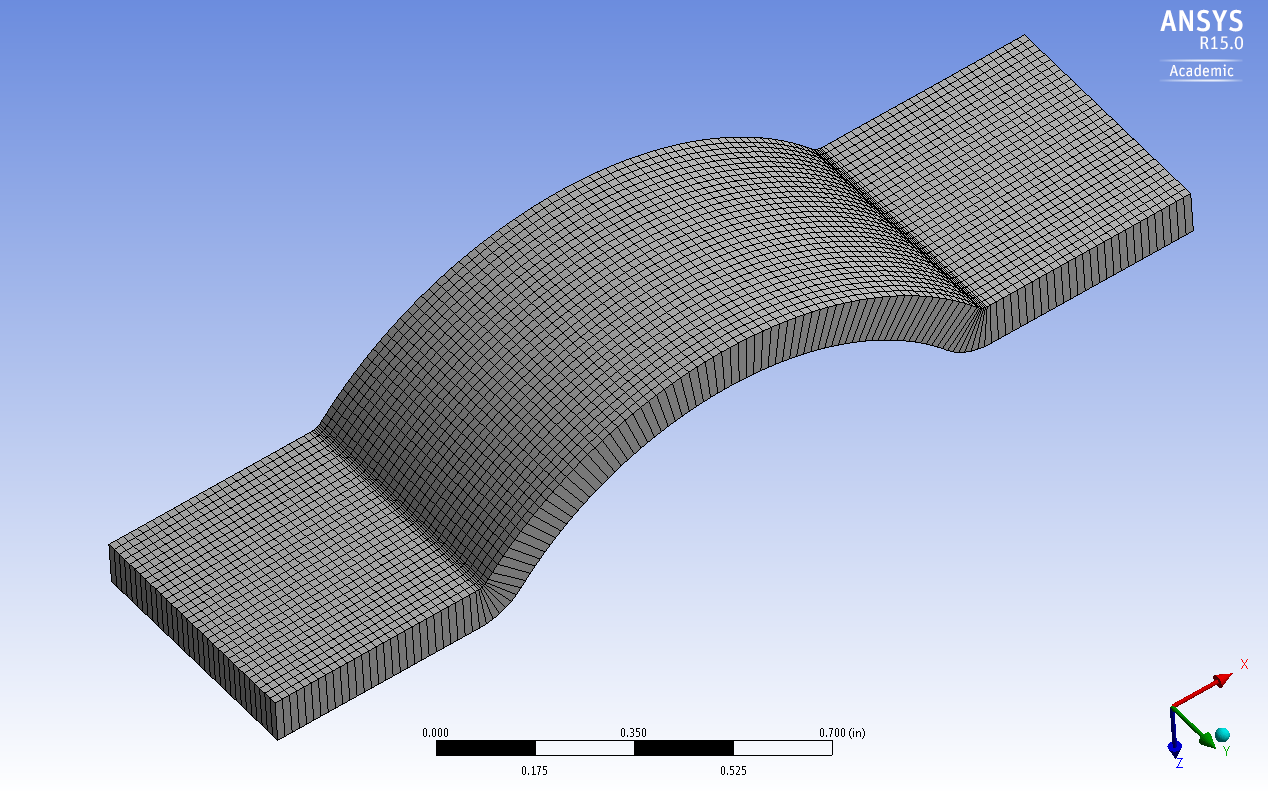
\includegraphics[width=1\textwidth]{./figures/fea/fea-mechanical-mesh-thick-shell}
\caption{The mesh as viewed when the shell elements are given a thickness.}
\label{fig:fea-mechanical-mesh-thick-shell}
\end{figure}

\begin{figure}[htp]
\centering
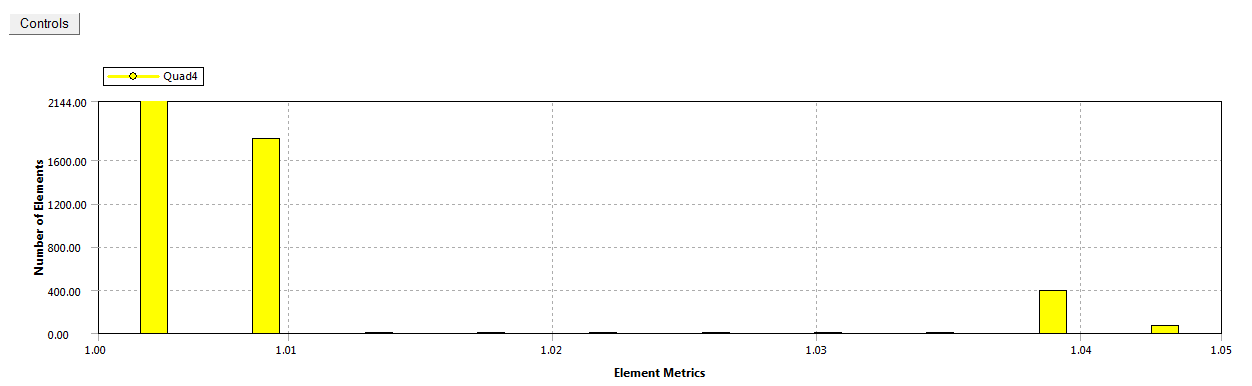
\includegraphics[width=1\textwidth]{./figures/fea/fea-mechanical-mesh-metrics-histogram}
\caption{A histogram of the aspect ratio of mesh elements.}
\label{fig:fea-mechanical-mesh-metrics-histogram}
\end{figure}

\clearpage

\subsection{ACP Setup}

%%% ACP Mesh Overview

\begin{figure}[htp]
\centering
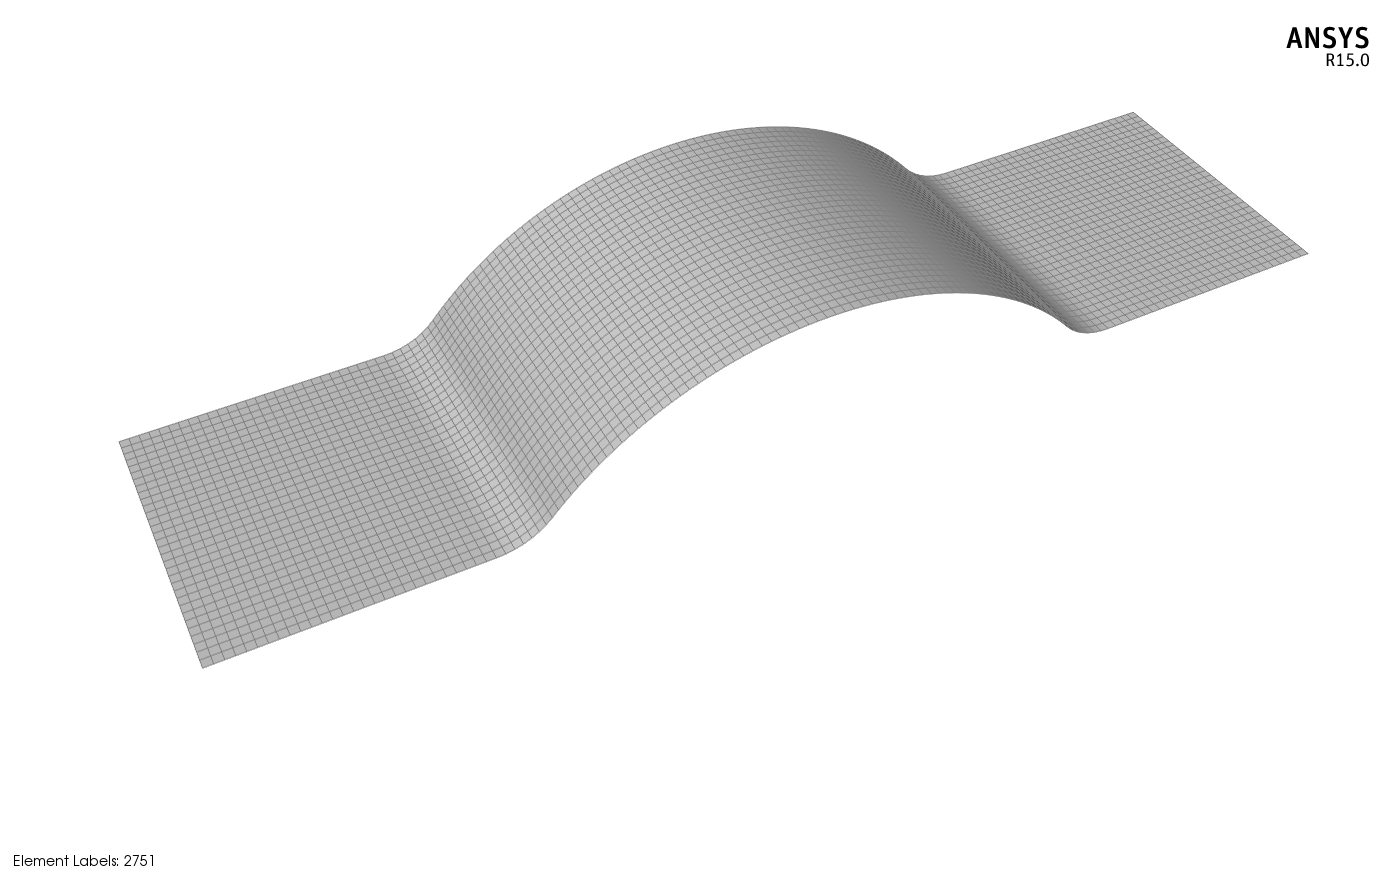
\includegraphics[width=1\textwidth]{./figures/fea/fea-acp-mesh-overview}
\caption{The mesh imported from \textit{ANSYS Mechanical} into \textit{ACP}.}
\label{fig:fea-acp-mesh-overview}
\end{figure}

%%% Control Tree

\begin{figure}[htp]
\centering
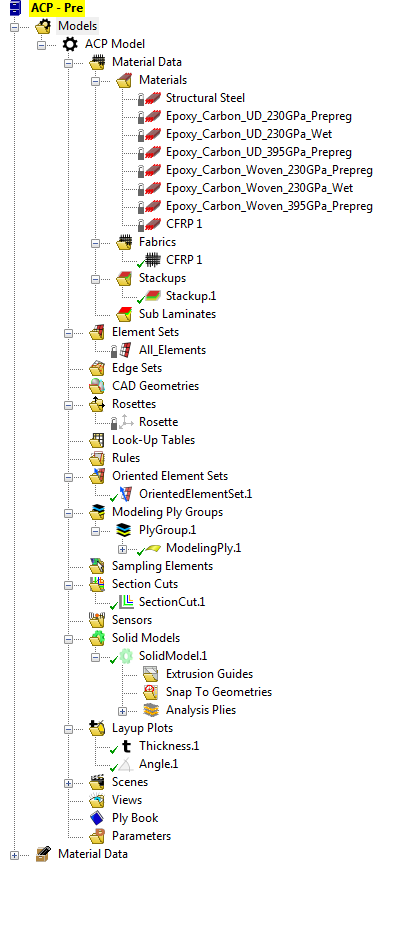
\includegraphics[width=0.25\textwidth]{./figures/fea/fea-acp-tree}
\caption{\textit{ACP}'s configuration tree.}
\label{fig:fea-acp-tree}
\end{figure}

%%% Fabric Properties

\begin{figure}[htp]
\centering
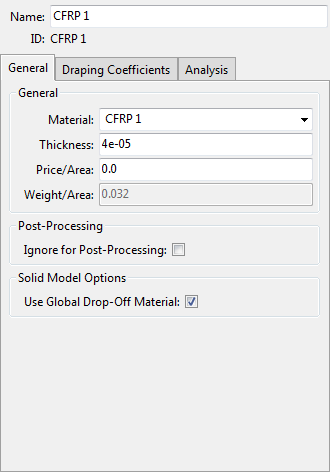
\includegraphics[width=0.5\textwidth]{./figures/fea/fea-acp-fabric-prorties-general}
\caption{General fabric proprerties used for FEA.}
\label{fig:fea-acp-fabric-prorties-general}
\end{figure}

\begin{figure}[htp]
\centering
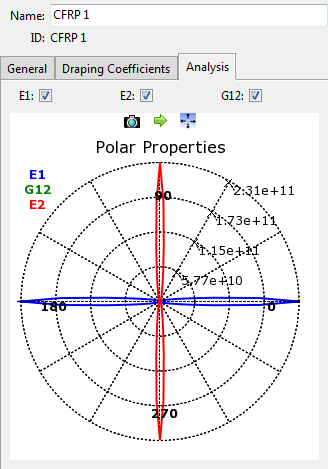
\includegraphics[width=0.5\textwidth]{./figures/fea/fea-acp-fabric-properties-polar}
\caption{Orthotropic fabric properites plotted in polar coordinates.}
\label{fig:fea-acp-fabric-properties-polar}
\end{figure}

%%% Stackup Properties

\begin{figure}[htp]
\centering
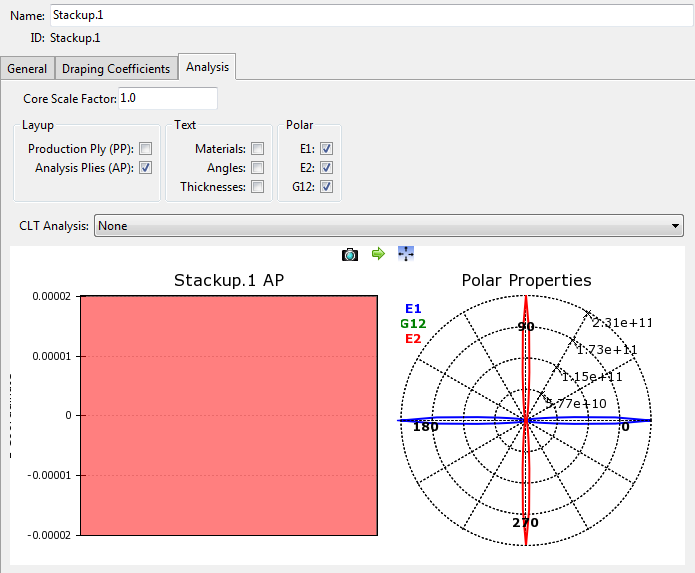
\includegraphics[width=0.5\textwidth]{./figures/fea/fea-acp-stackup-proprties}
\caption{Stackup proprerties used for FEA.}
\label{fig:fea-acp-stackup-proprties}
\end{figure}

%%% Oriented Elements Properties

\begin{figure}[htp]
\centering
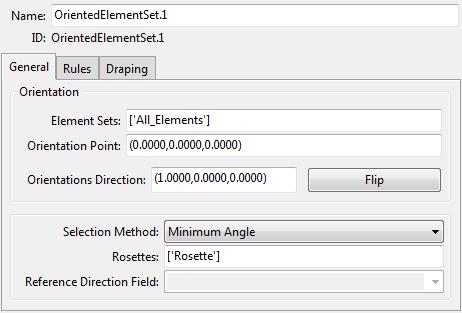
\includegraphics[width=0.5\textwidth]{./figures/fea/fea-acp-oriented-element-properties}
\caption{Oriented element properties used to establish a reference direction.}
\label{fig:fea-acp-oriented-element-properties}
\end{figure}

\begin{figure}[htp]
\centering
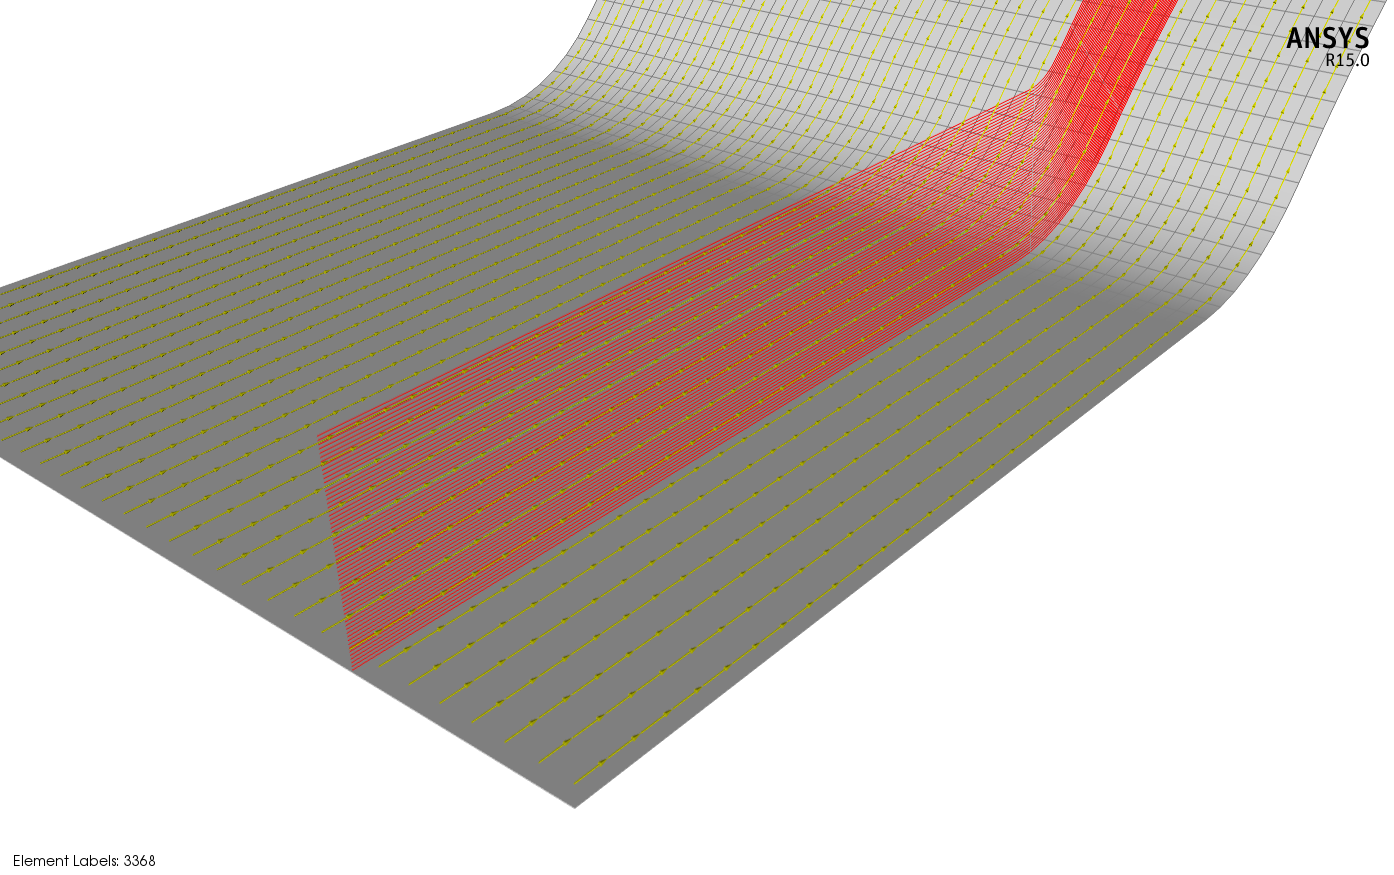
\includegraphics[width=1\textwidth]{./figures/fea/fea-acp-reference-direction}
\caption{Reference direction vector displayed in the finite element model.}
\label{fig:fea-acp-reference-direction}
\end{figure}

\begin{figure}[htp]
\centering
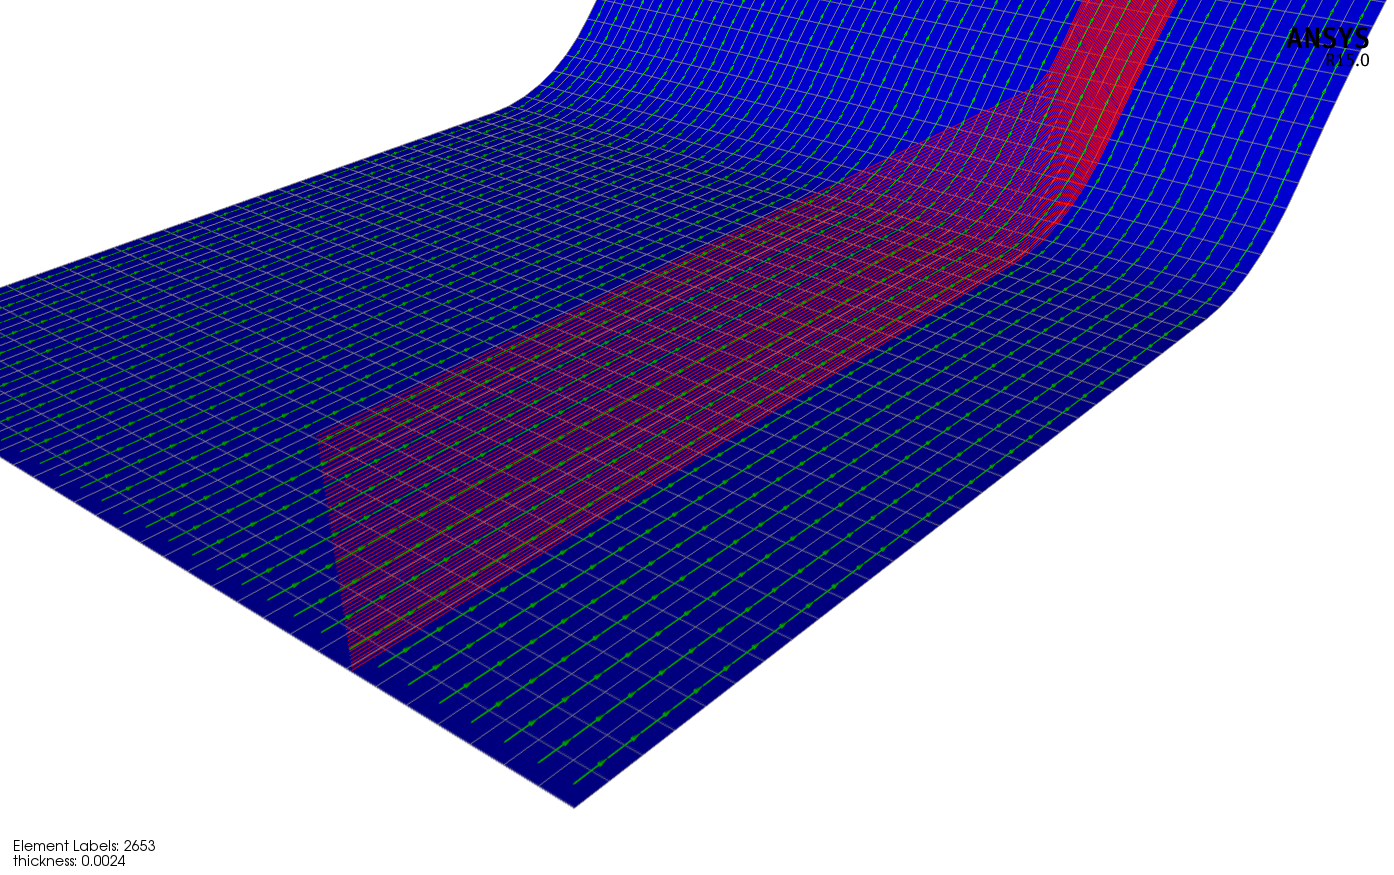
\includegraphics[width=1\textwidth]{./figures/fea/fea-acp-fiber-direction}
\caption{Fiber direction vector displayed in the finite element model.}
\label{fig:fea-acp-fiber-direction}
\end{figure}

%%% Modeling Plys

\begin{figure}[htp]
\centering
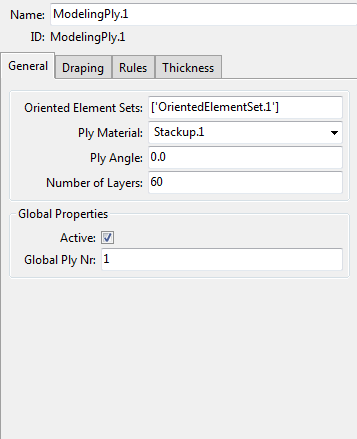
\includegraphics[width=0.5\textwidth]{./figures/fea/fea-acp-modeling-ply-properties}
\caption{Ply properties used for FEA.}
\label{fig:fea-acp-modeling-ply-properties}
\end{figure}

\begin{figure}[htp]
\centering
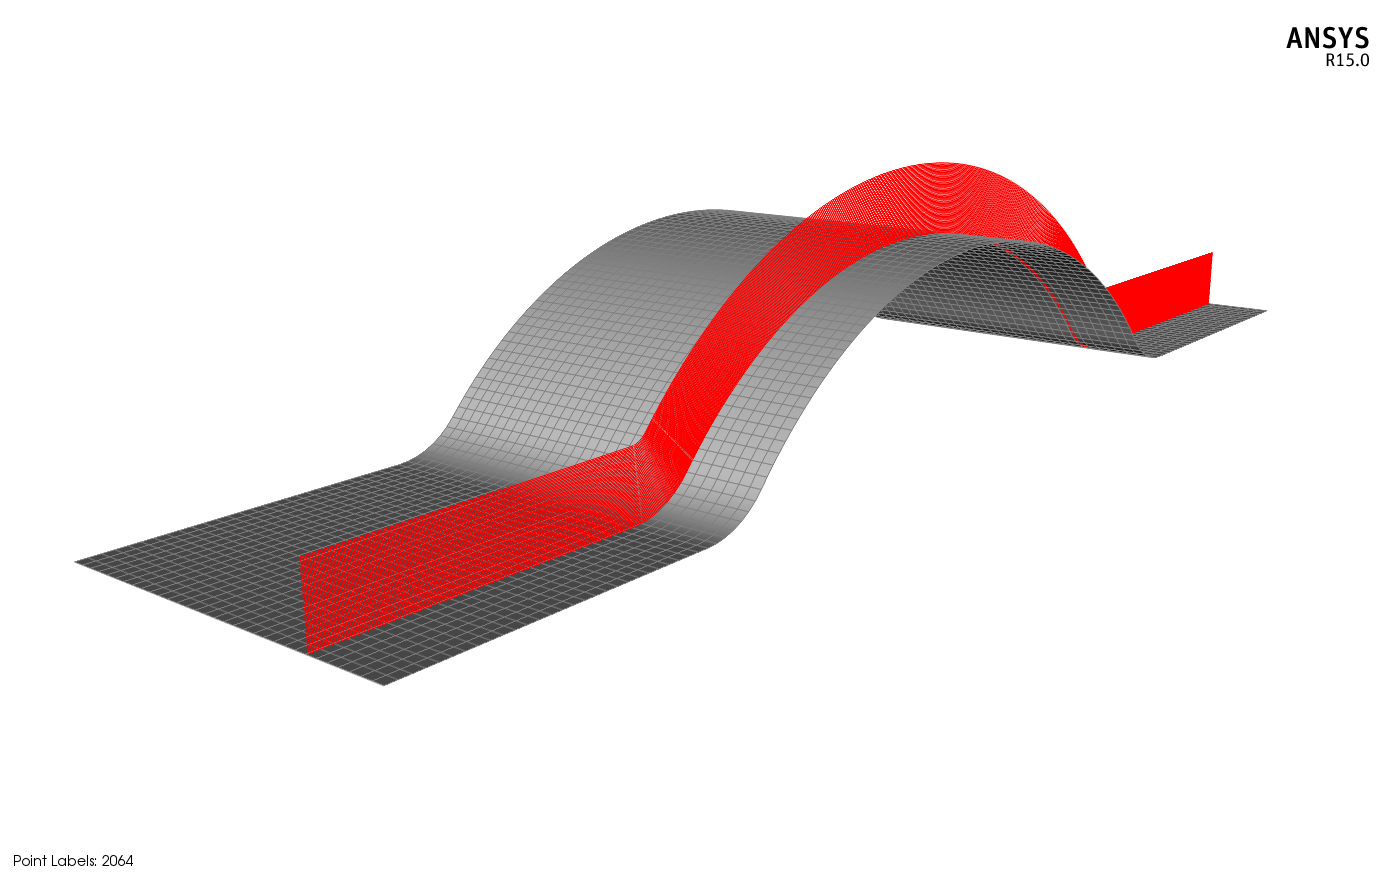
\includegraphics[width=1\textwidth]{./figures/fea/fea-acp-ply-scaling}
\caption{A ply scaling representation of the composite finitie element model.}
\label{fig:fea-acp-ply-scaling}
\end{figure}

%%% Solid body representation

\begin{figure}[htp]
\centering
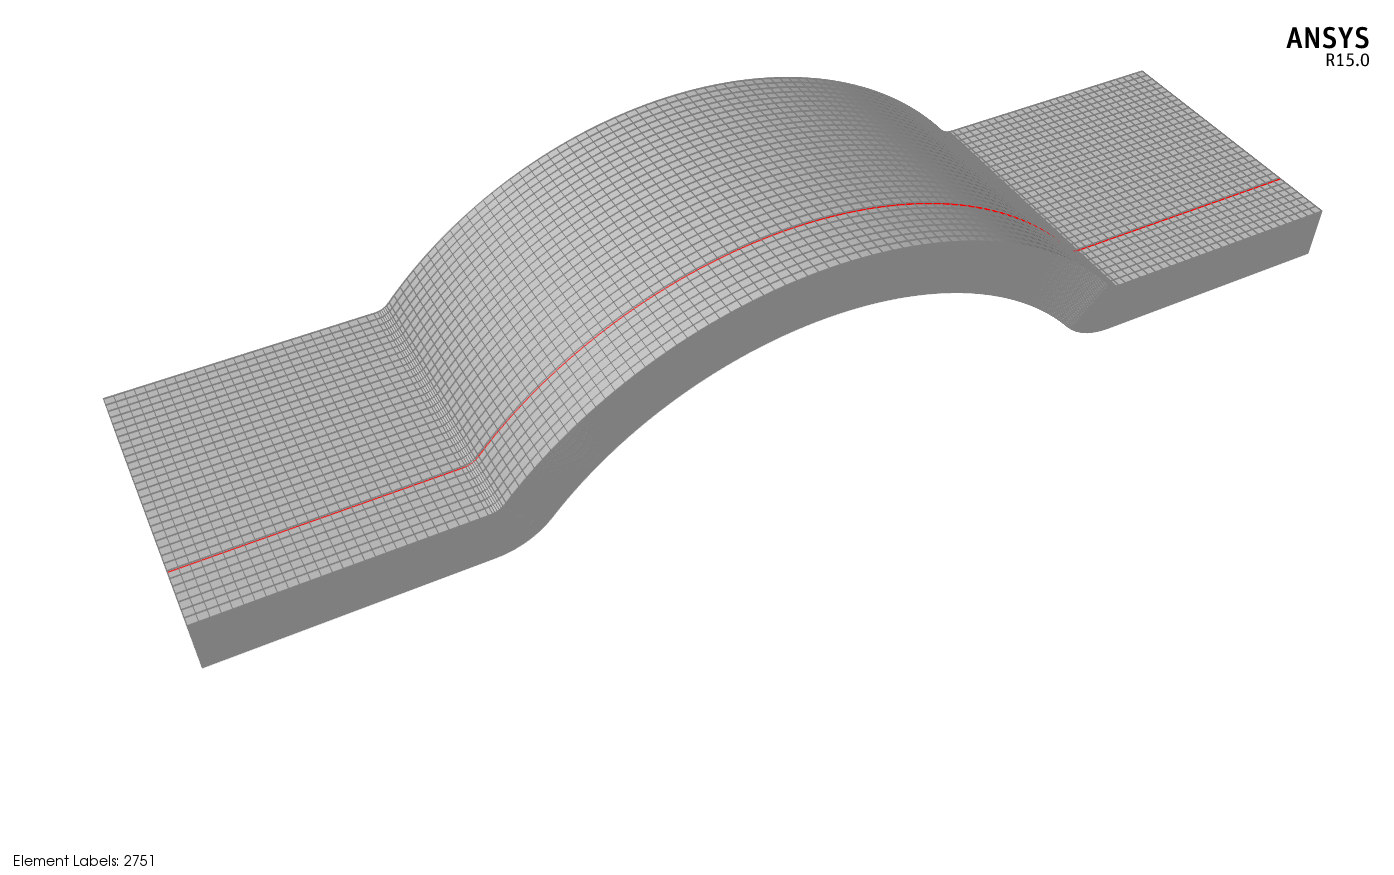
\includegraphics[width=1\textwidth]{./figures/fea/fea-acp-solidmodel-mesh}
\caption{Mesh overview of the composite model in \textit{ACP} with a solid-body display state applied.}
\label{fig:fea-acp-solidmodel-mesh}
\end{figure}

\begin{figure}[htp]
\centering
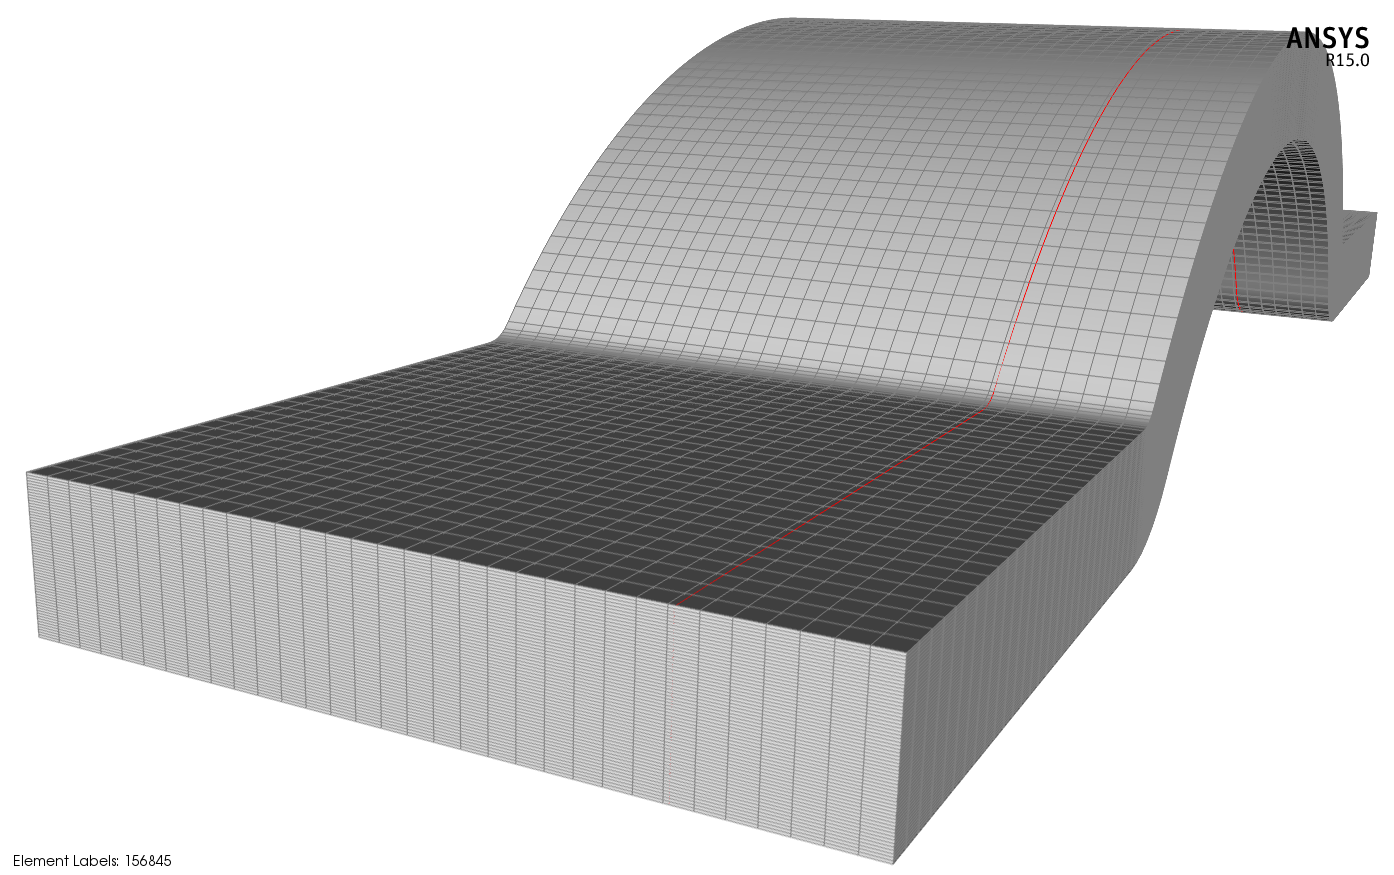
\includegraphics[width=1\textwidth]{./figures/fea/fea-acp-solidmodel-closeup}
\caption{Mesh overview of the composite model in \textit{ACP} with a solid-body display state applied.}
\label{fig:fea-acp-solidmodel-closeup}
\end{figure}

\clearpage

\subsection{Failure Criteria}

\begin{figure}[htp]
\centering
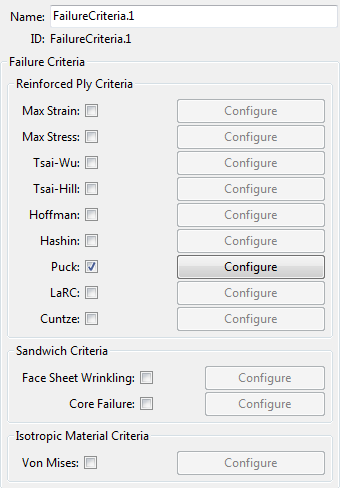
\includegraphics[width=0.5\textwidth]{./figures/fea/fea-acp-failure-criteria-definition}
\caption{Composite failure criteria available in \textit{ACP}.}
\label{fig:fea-acp-failure-criteria-definition}
\end{figure}

\begin{figure}[htp]
\centering
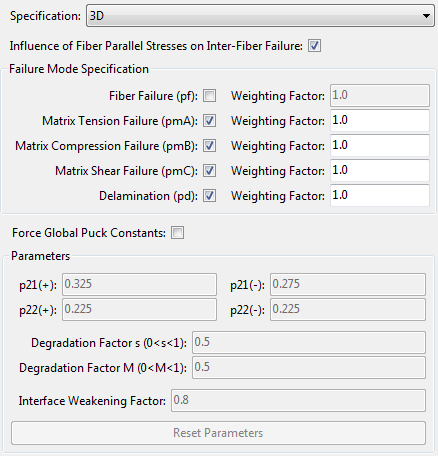
\includegraphics[width=0.5\textwidth]{./figures/fea/fea-acp-puck-failure-criterion}
\caption{The Puck failure criterion properties applied to the finite element model.}
\label{fig:fea-acp-puck-failure-criterion}
\end{figure}

\clearpage

\subsection{Solid Body FEA Comparison}

\subsubsection{Physics Models}

\clearpage

\subsubsection{Geometry}

\begin{figure}[htp]
\centering
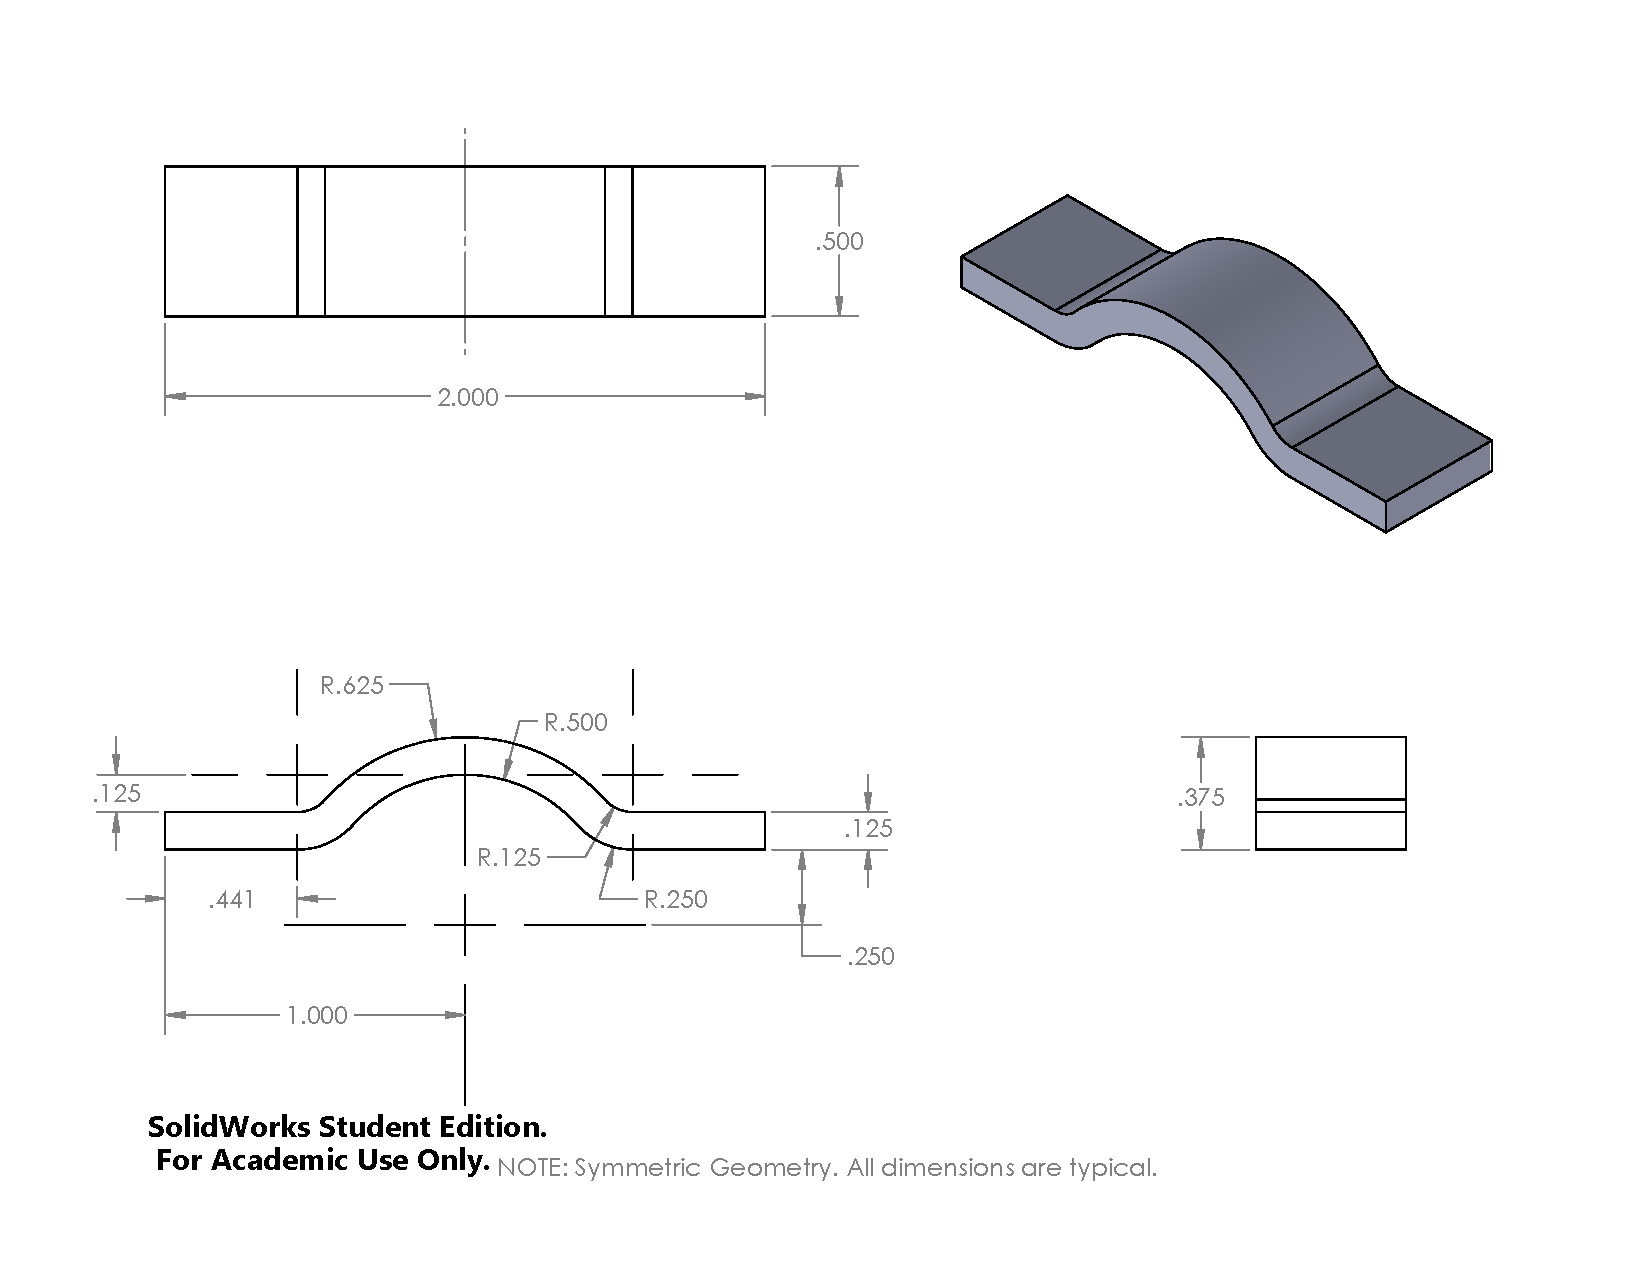
\includegraphics[width=1\textwidth]{./figures/fea/fea-body-geometry}
\caption{A \emph{SolidWorks} drawing of the solid body used for the comparison FEA.}
\label{fig:fea-acp-puck-failure-criterion}
\end{figure}

\clearpage

\subsubsection{Material Properties}

\clearpage

\subsubsection{Mesh}

\begin{figure}[htp]
\centering
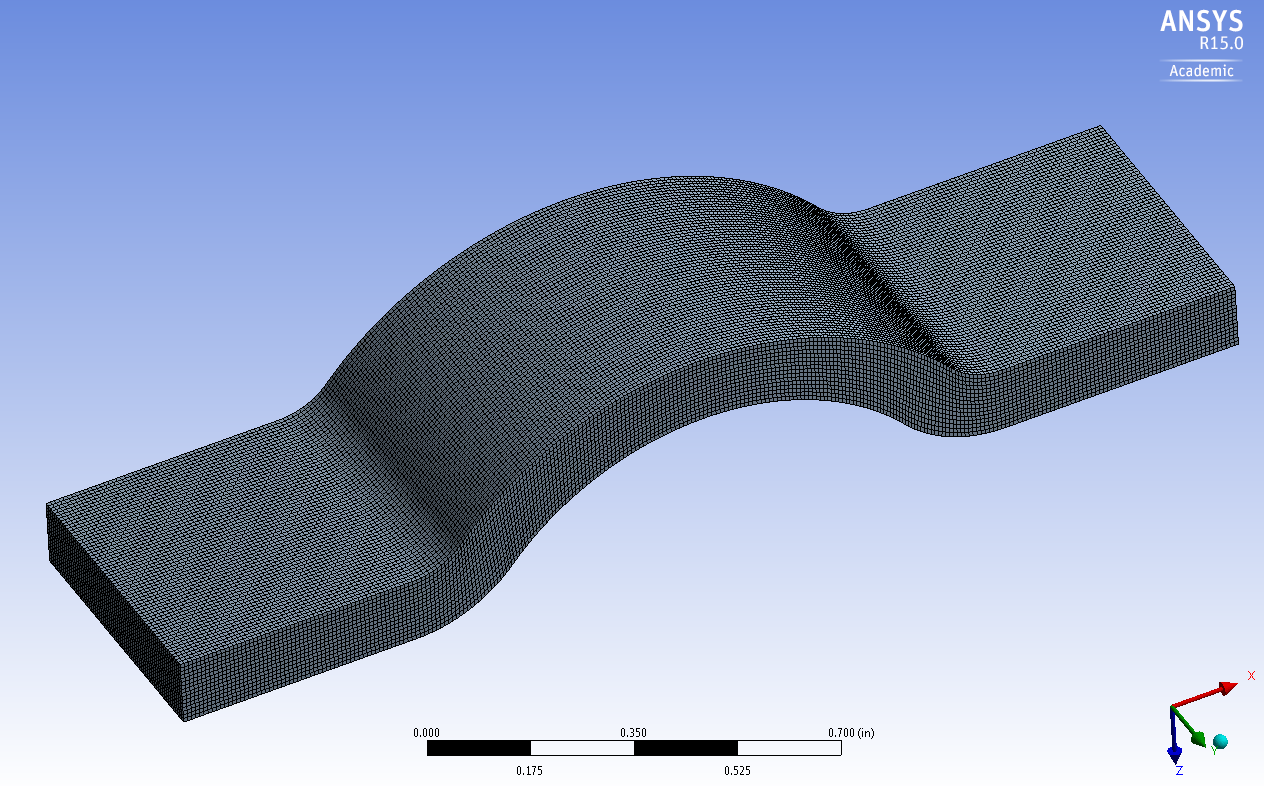
\includegraphics[width=1\textwidth]{./figures/fea/fea-solid-mesh-overview}
\caption{An overview of the mesh used for the standard FEA.}
\label{fig:fea-solid-mesh-overview}
\end{figure}

\begin{figure}[htp]
\centering
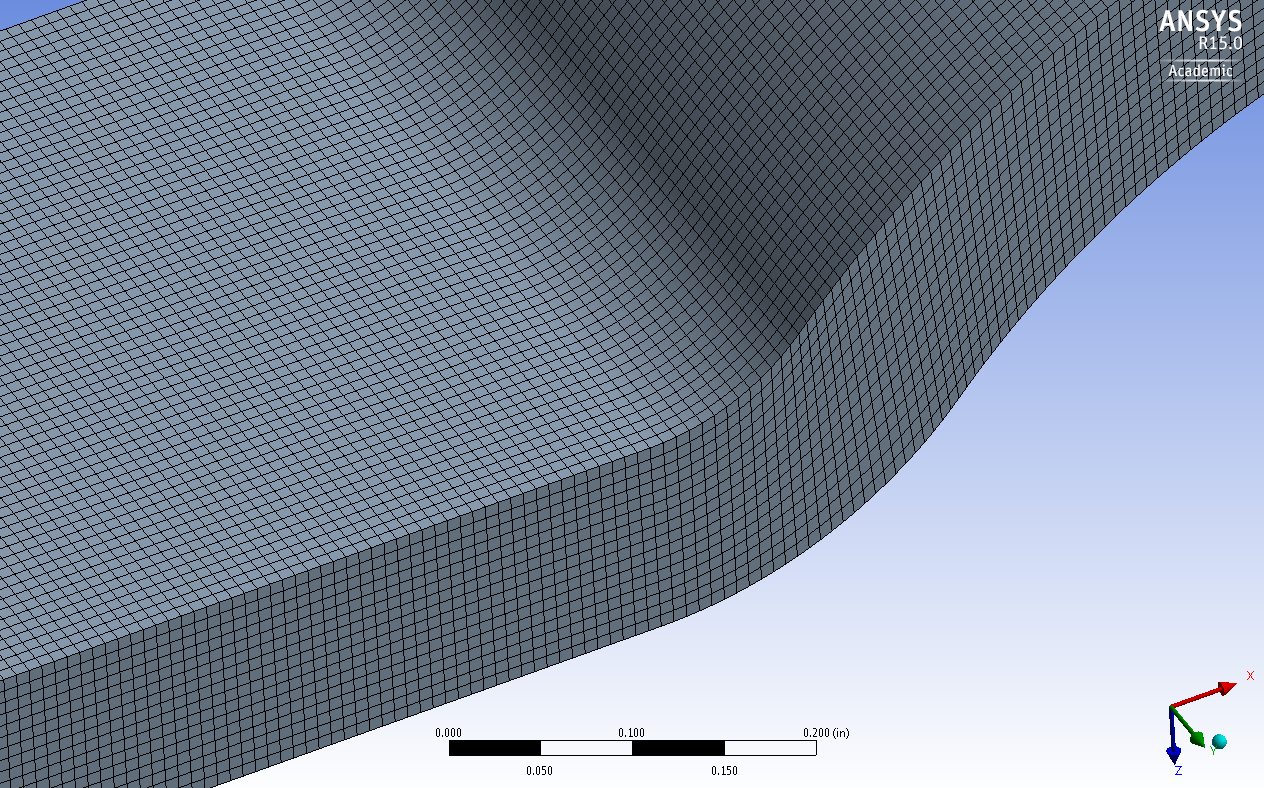
\includegraphics[width=1\textwidth]{./figures/fea/fea-solid-mesh-closeup}
\caption{A close-up of the mesh used for the standard FEA.}
\label{fig:fea-solid-mesh-closeup}
\end{figure}

\begin{figure}[htp]
\centering
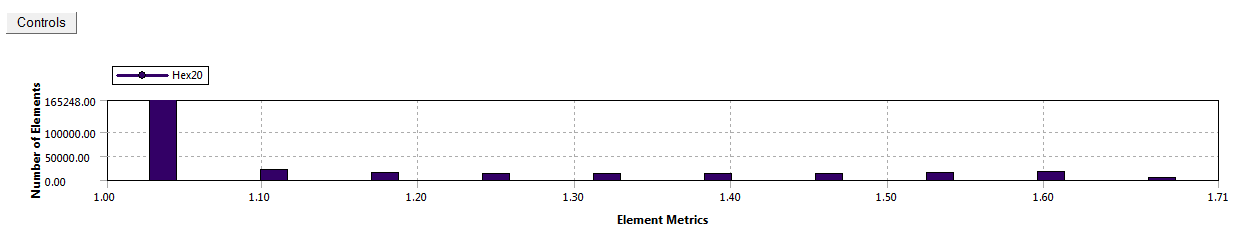
\includegraphics[width=1\textwidth]{./figures/fea/fea-solid-mesh-metrics}
\caption{Mesh statistics for the solid model FEA.}
\label{fig:fea-solid-mesh-metrics}
\end{figure}

\clearpage

\subsubsection{Loads and Boundary Conditions}

\begin{figure}[htp]
\centering
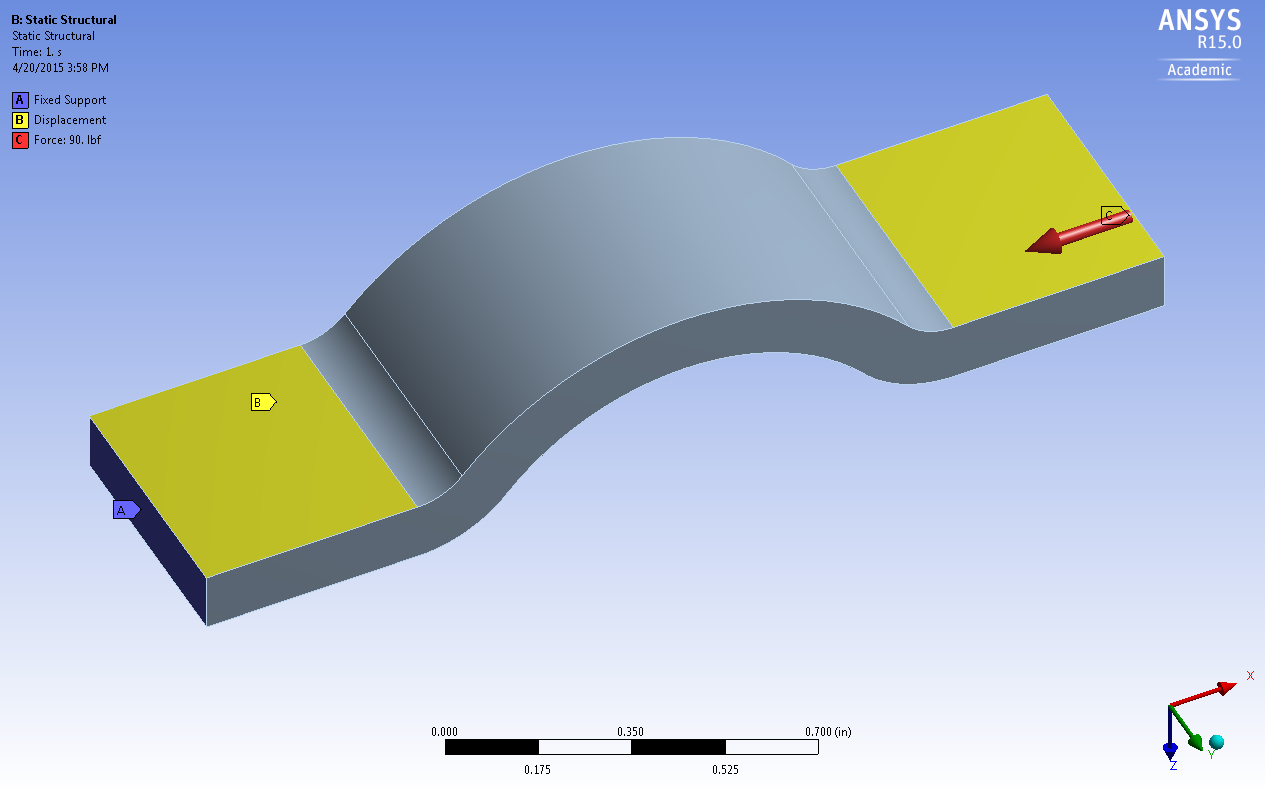
\includegraphics[width=1\textwidth]{./figures/fea/fea-solid-loads-bcs}
\caption{Loads and boundary conditions applied to the solid model fea.}
\label{fig:fea-solid-loads-bcs}
\end{figure}

\begin{figure}[htp]
\centering
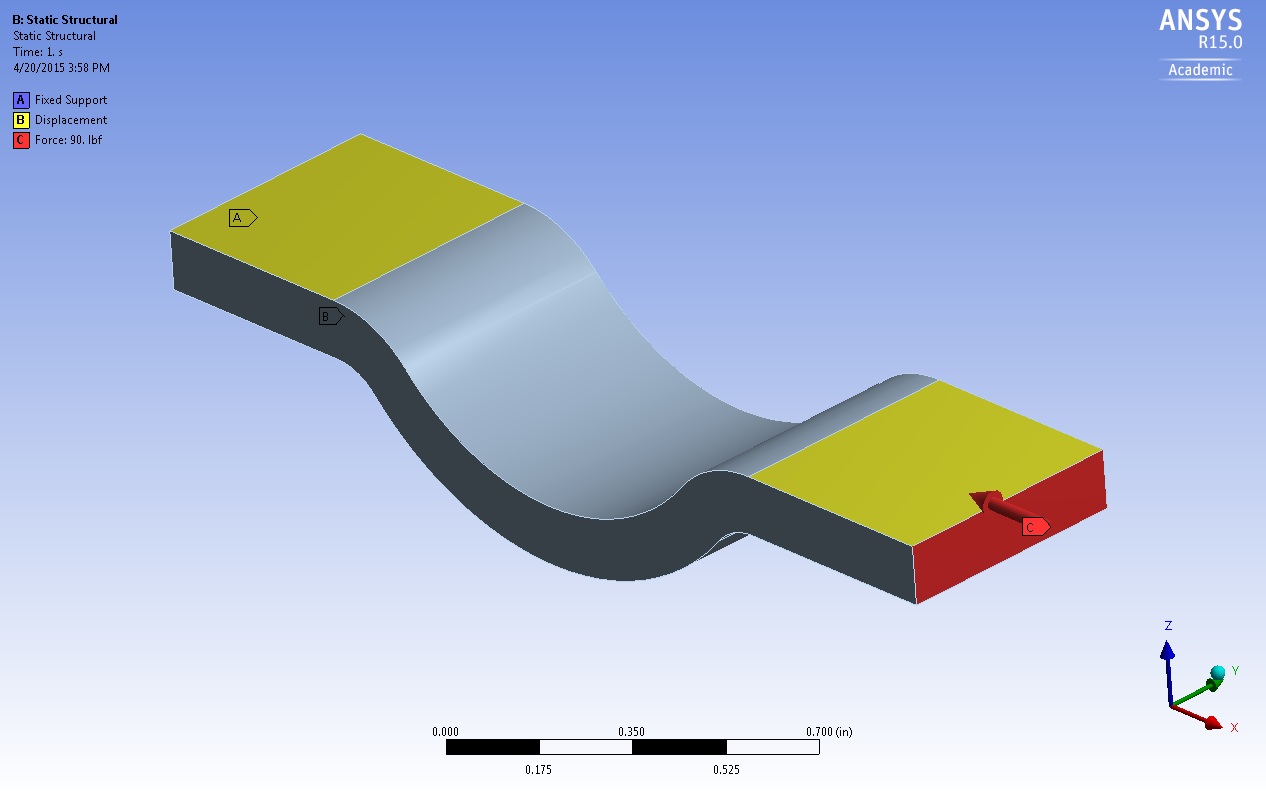
\includegraphics[width=1\textwidth]{./figures/fea/fea-solid-loads-bcs-3}
\caption{Another view of loads and boundary conditions applied to the solid model fea.}
\label{fig:fea-solid-loads-bcs-3}
\end{figure}

\clearpage

\subsubsection{Results}

%%% ABS

\begin{figure}[htp]
\centering
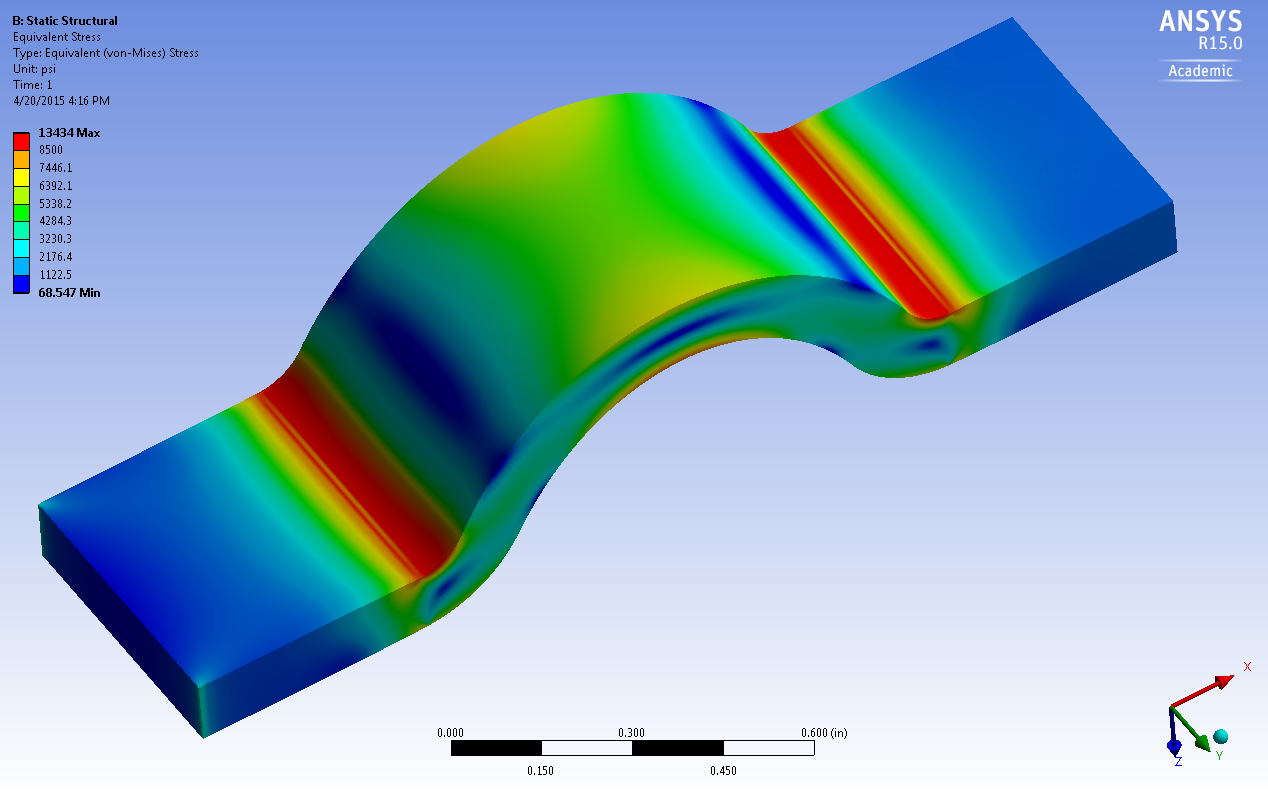
\includegraphics[width=1\textwidth]{./figures/fea/fea-solid-vms-top}
\caption{A top-isometric view of von-mises stress for a solid-body ABS analysis.}
\label{fig:fea-solid-vms-top}
\end{figure}

\begin{figure}[htp]
\centering
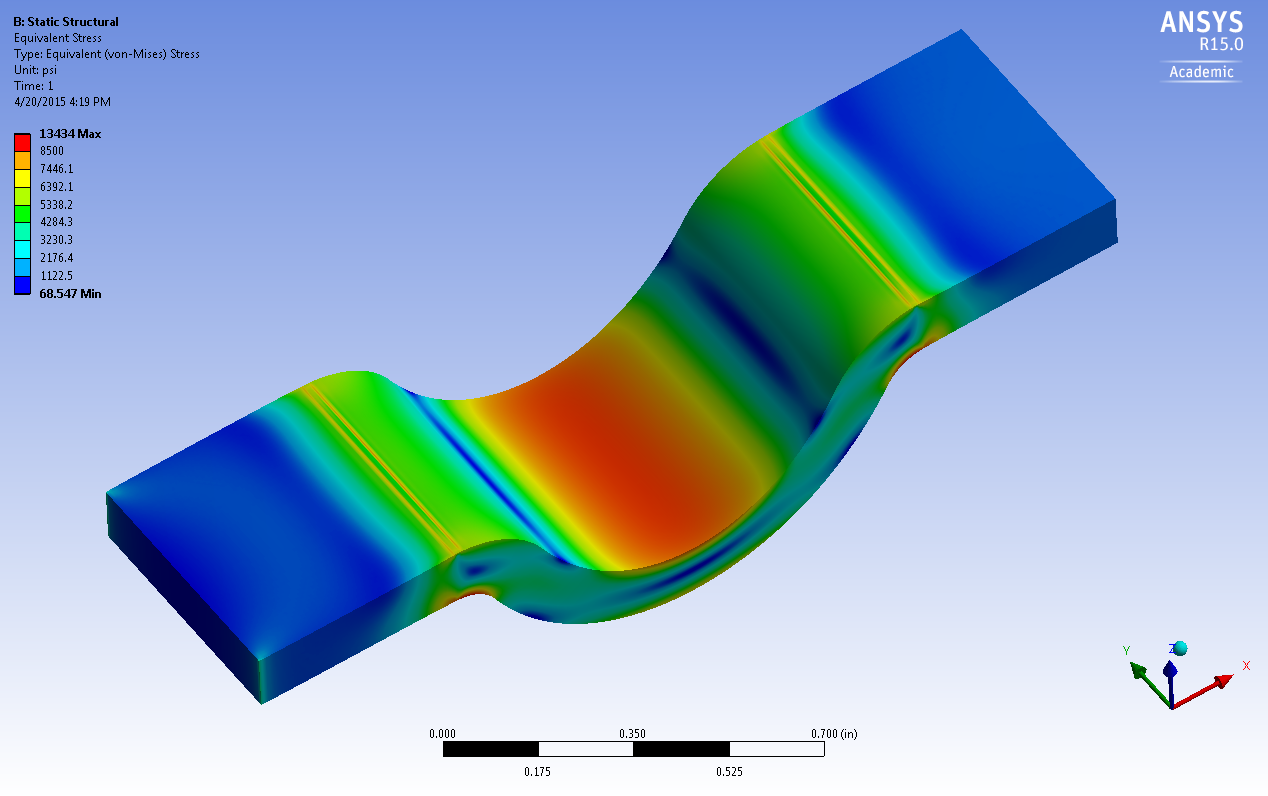
\includegraphics[width=1\textwidth]{./figures/fea/fea-solid-vms-bottom}
\caption{A bottom -isometric view of von-mises stress for a solid-body ABS analysis.}
\label{fig:fea-solid-vms-bottom}
\end{figure}

%%% Aluminum

%stresses

\begin{figure}[htp]
\centering
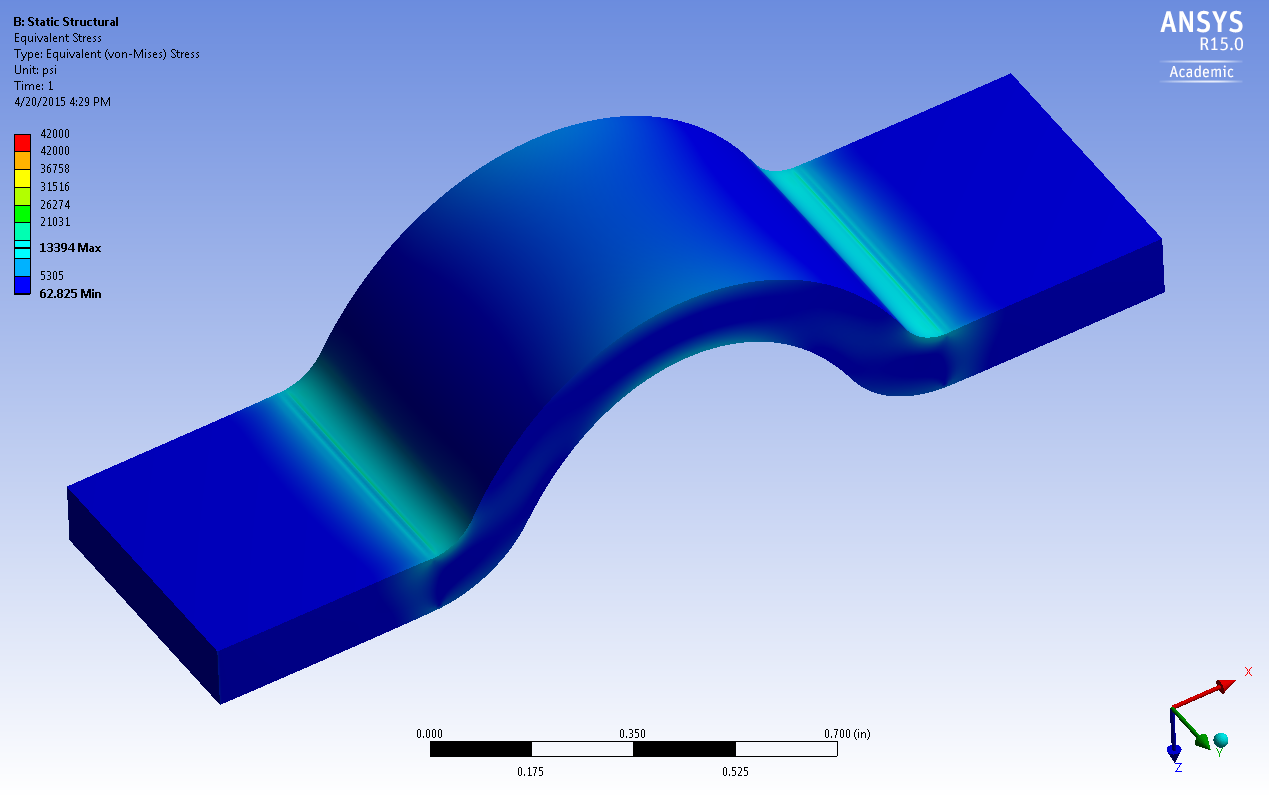
\includegraphics[width=1\textwidth]{./figures/fea/fea-solid-al-vms-top}
\caption{A top-isometric view of von-mises stress for a solid-body aluminum analysis.}
\label{fig:fea-solid-al-vms-top}
\end{figure}

\begin{figure}[htp]
\centering
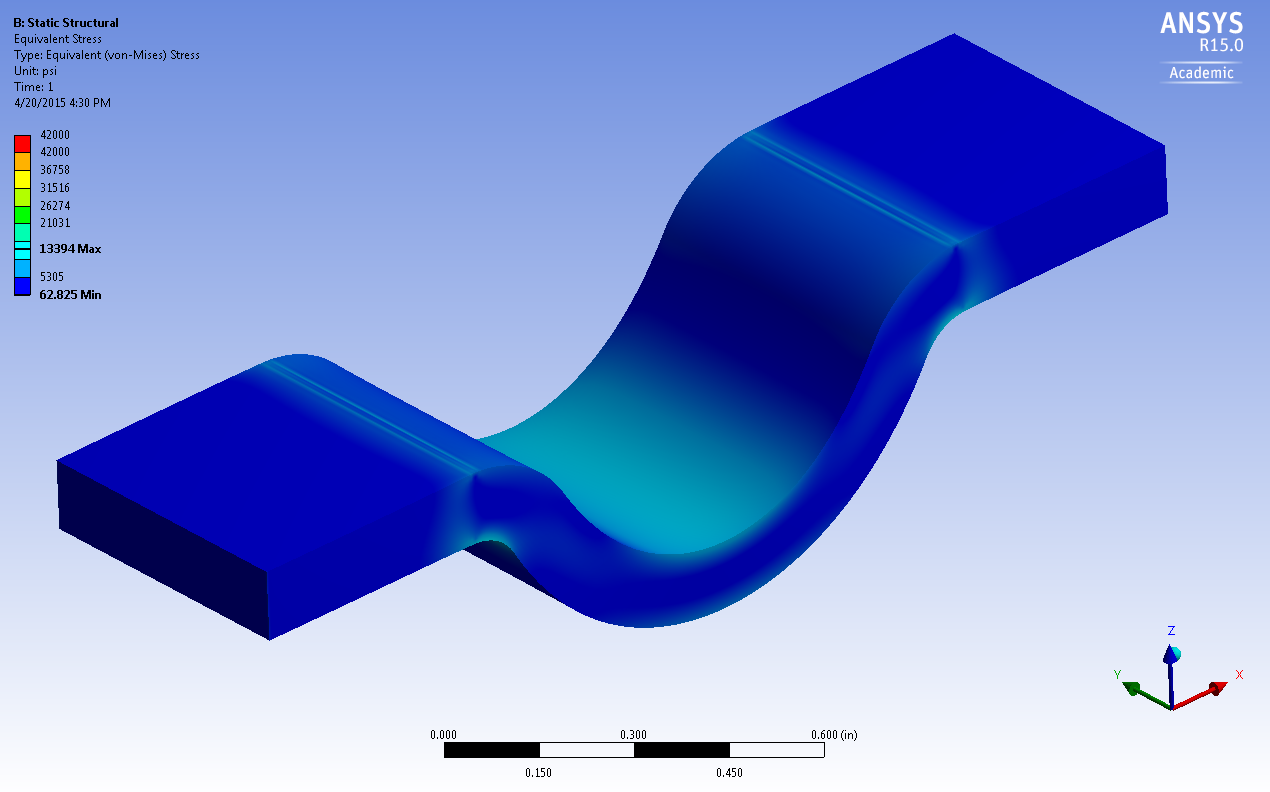
\includegraphics[width=1\textwidth]{./figures/fea/fea-solid-al-vms-bottom}
\caption{A bottom -isometric view of von-mises stress for a solid-body aluminum analysis.}
\label{fig:fea-solid-al-vms-bottom}
\end{figure}

%stresses

\begin{figure}[htp]
\centering
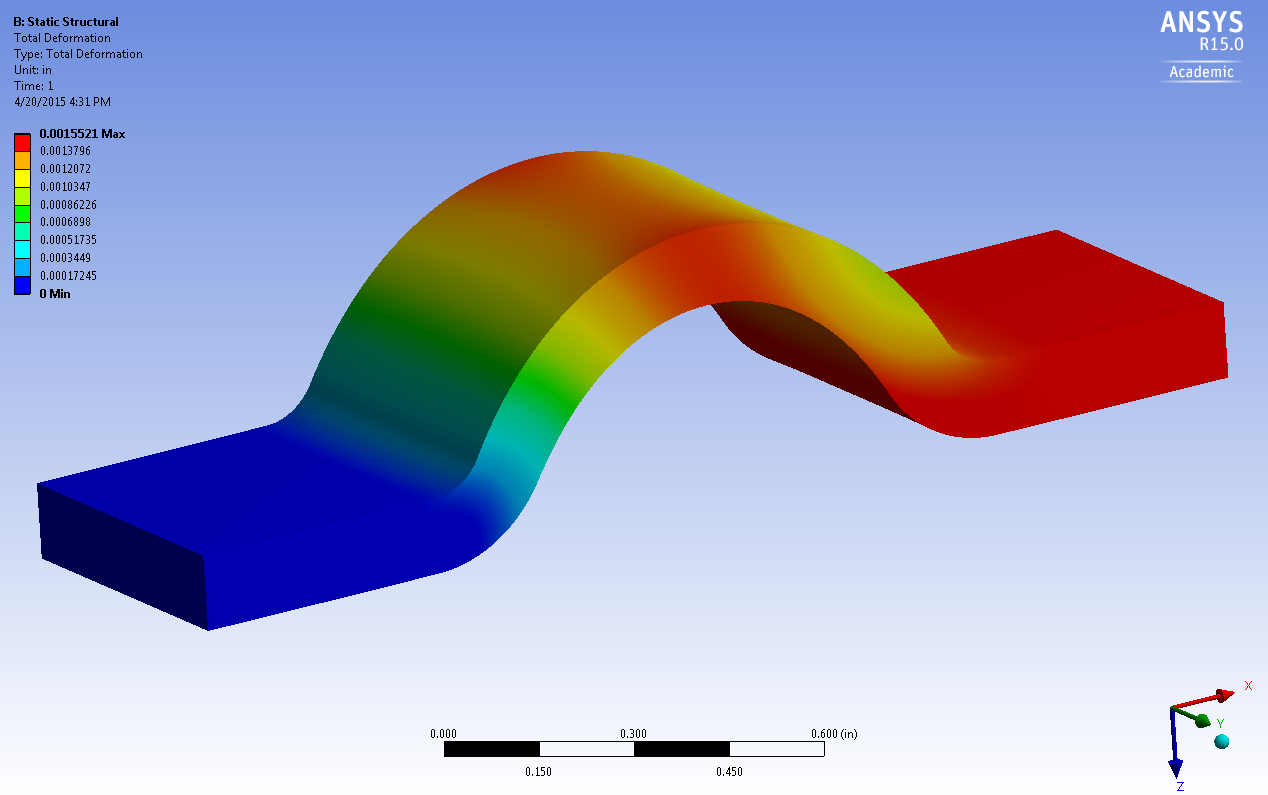
\includegraphics[width=1\textwidth]{./figures/fea/fea-solid-al-def-tot}
\caption{Total deformation from the solid-body aluminum analysis.}
\label{fig:fea-solid-al-def-tot}
\end{figure}

\begin{figure}[htp]
\centering
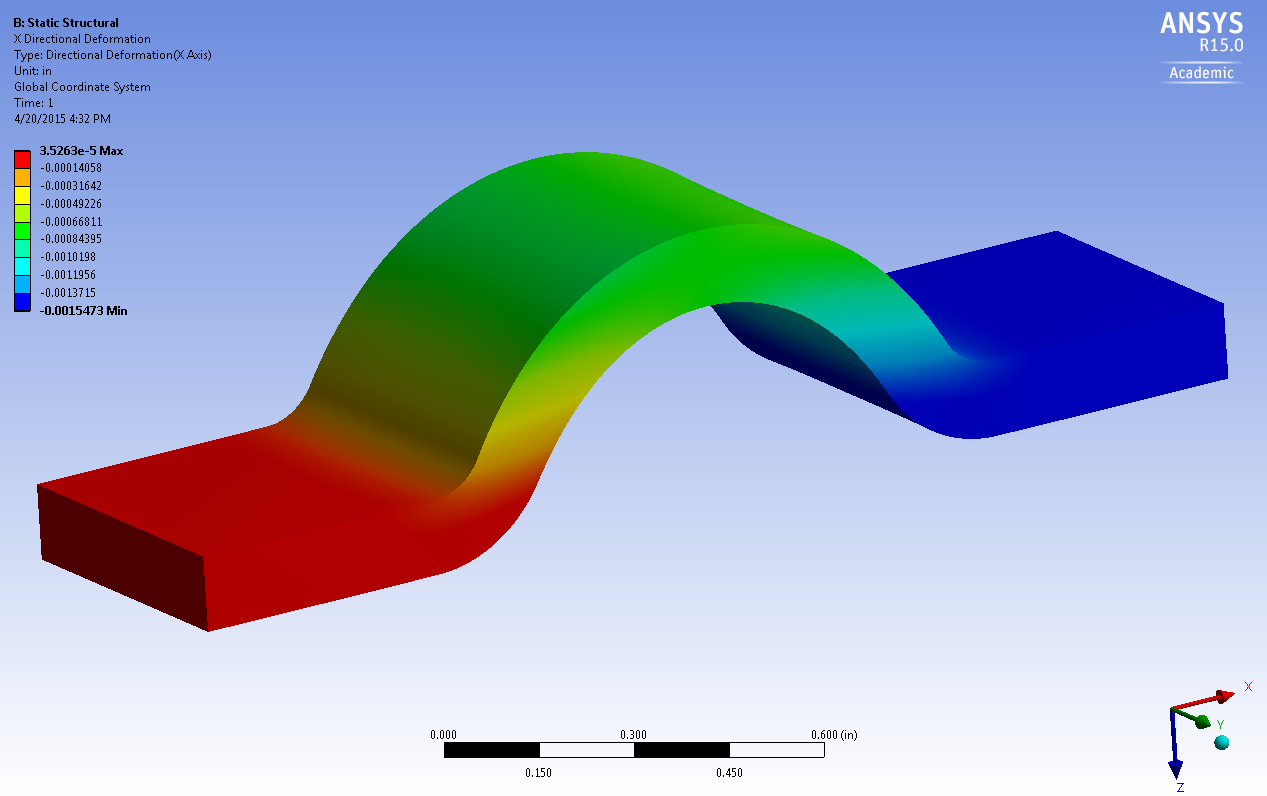
\includegraphics[width=1\textwidth]{./figures/fea/fea-solid-al-def-x}
\caption{X direction deformation from the solid-body aluminum analysis.}
\label{fig:fea-solid-al-def-x}
\end{figure}

\begin{figure}[htp]
\centering
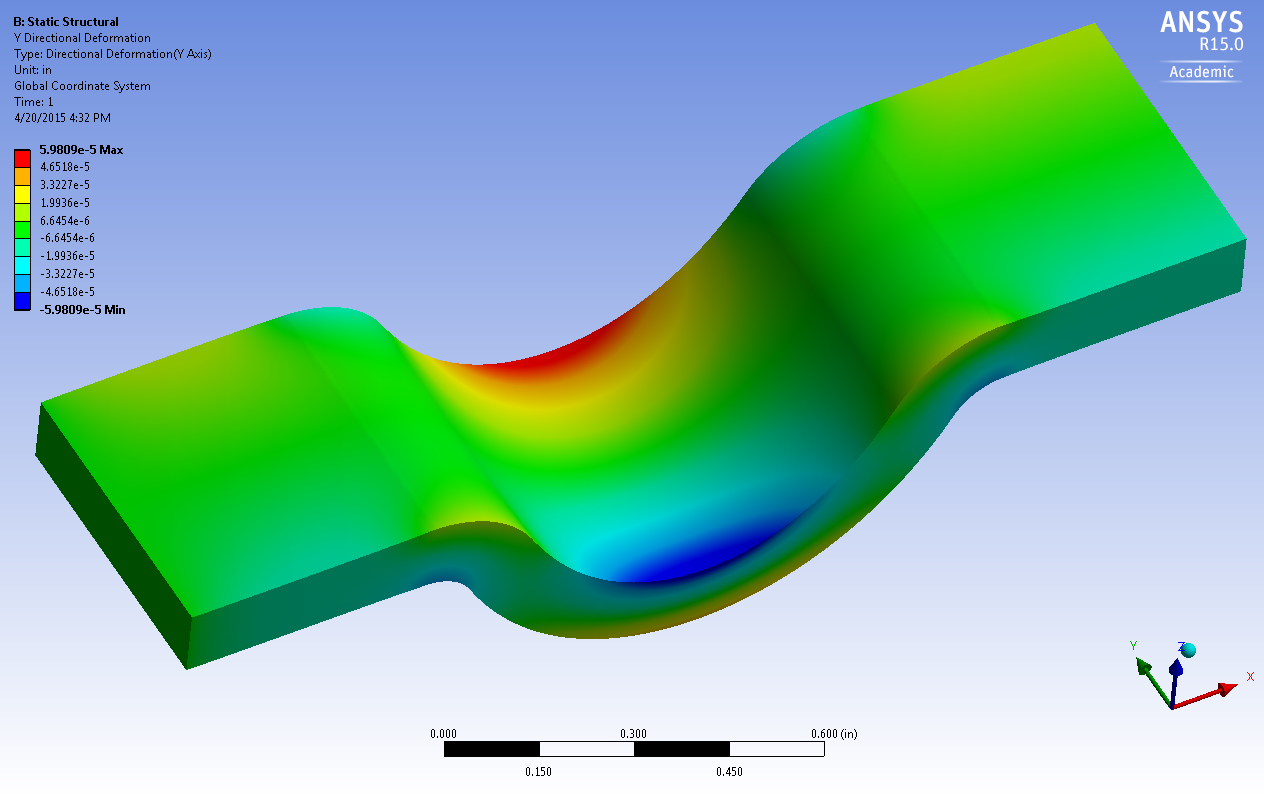
\includegraphics[width=1\textwidth]{./figures/fea/fea-solid-al-def-y}
\caption{Y direction deformation from the solid-body aluminum analysis.}
\label{fig:fea-solid-al-def-y}
\end{figure}

\begin{figure}[htp]
\centering
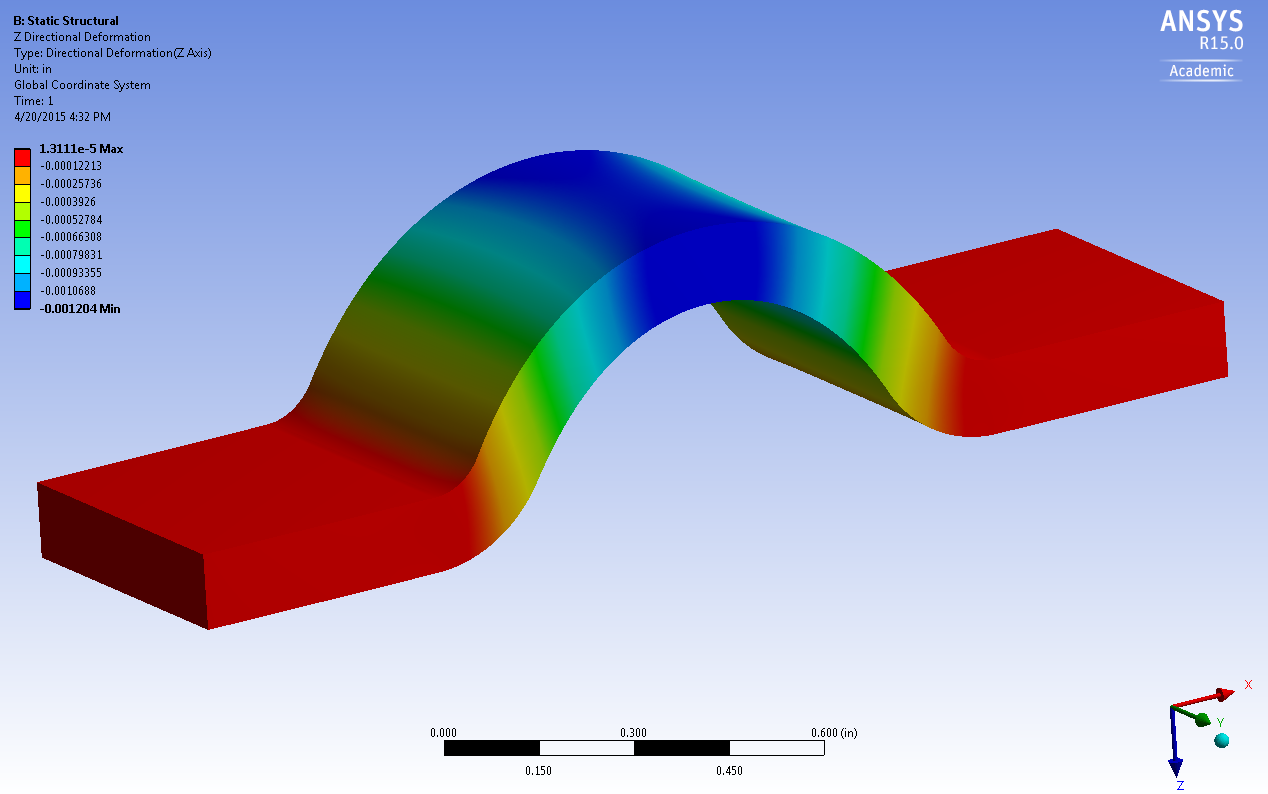
\includegraphics[width=1\textwidth]{./figures/fea/fea-solid-al-def-z}
\caption{Z direction deformation from the solid-body aluminum analysis.}
\label{fig:fea-solid-al-def-z}
\end{figure}

\clearpage

\subsection{Conclusions from FEA}

insert conclusions / future suggestions here

\clearpage